% vim: set spell spelllang=es syntax=tex :

\documentclass[11pt,a4paper,spanish]{beamer}

\usepackage[spanish]{babel}

\usepackage[utf8]{inputenc}

\usepackage{graphicx}

\usepackage{subcaption} %Para Subfigure

\usepackage{caption} %Para captions en las figuras sin prefijo

\usepackage{ccicons}

\usepackage{url}

\usepackage{babelbib}

\usefonttheme{serif}

\setlength{\parskip}{1.5mm}

\usetheme{Rochester}
\usecolortheme{whale}

%\usetheme{Warsaw}

\beamertemplatenavigationsymbolsempty

\setbeamertemplate{background canvas}{
    \raisebox{-0.99\paperheight}[0pt][0pt]{
        \makebox[\paperwidth]{
            \null
            \hspace{-1em}
            
\includegraphics[width=0.09\paperwidth]{logos/fai.pdf}
            \hspace{0.8\paperwidth}
            %\hfill
            \hspace{-1em}
            \includegraphics[width=0.09\paperwidth]{logos/uncoma.pdf}
            }
    }
}

\title{Introducción a\\
\textbf{Introducción a la Computación}}

\author{}

\date{}

\defbeamertemplate{footline}{centered page number}
{
    \hspace*{\fill}
    \usebeamercolor[fg]{blue}
    \usebeamerfont{page number in head/foot}
    \insertpagenumber\,/\,\insertpresentationendpage
    \hspace*{\fill}\vskip2pt
}
\setbeamertemplate{footline}[centered page number]

\begin{document}

\begin{frame}[noframenumbering]

    \maketitle
    \centering
    \vspace{-8em}~
    \begin{figure}
    
\includegraphics[height=0.65\textheight]{img/ckitten.jpg}
        \captionsetup{textfont=tiny,labelformat=empty}
        \caption{\ccbysa\cite{ckitten}}
    \end{figure}

\end{frame}

\begin{frame}

    \frametitle{Temario}

\begin{itemize}

\item ¿Quiénes?

\item ¿Qué?

\item ¿Cuándo y dónde?

\item ¿Cómo?

\end{itemize}

\end{frame}

\begin{frame}

    \frametitle{Equipo de cátedra}

\begin{itemize}

\item Docentes a cargo:
    \begin{itemize}
        \item Marina Moran
        \item Rodrigo S. Cañibano
    \end{itemize}

\item Jefe de trabajos prácticos:
    \begin{itemize}
        \item Lucas Cavaliere
    \end{itemize}

\item Ayudantes:
    \begin{itemize}
        \item Santino Castagno
        \item Juan Mestica
        \item \emph{¿¿¿???}
    \end{itemize}
\end{itemize}

\end{frame}

\begin{frame}

    \frametitle{Temario de la materia}

\begin{enumerate}

    \setcounter{enumi}{-1}

    \item Historia de la computación.

    \item Representación de la información:
        \begin{itemize}
            \item Sistemas de Numeración, Unidades de Información,
                Representación Digital de Datos.
        \end{itemize}

    \item Organización de las Computadoras:
        \begin{itemize}
            \item Componentes y Arquitectura de una computadora, CPU, Memoria,
                Dispositivos, Ejecución de Programas.
        \end{itemize}

    \item Software:
        \begin{itemize}
            \item Compiladores e intérpretes, Lenguajes de Programación,
                Sistemas Operativos.
        \end{itemize}

    \item Redes:
        \begin{itemize}
            \item Internet, Ruteo, Servicio de Nombres de Dominio.
        \end{itemize}

\end{enumerate}

\end{frame}

\begin{frame}

    \frametitle{Página de la materia}
    \framesubtitle{\url{https://se.fi.uncoma.edu.ar/ic/}}

\begin{itemize}
    \item Últimas novedades.
    \item Información de contacto de los docentes.
    \item Horarios.
    \item Programa de la materia.
    \item Link a las clases grabadas.
    \item Trabajos prácticos.
    \item Preguntas frecuentes (FAQ).
    \item Link a los foros de \emph{PedCo}:
        \begin{itemize}
            \item Novedades.
            \item Consultas.
        \end{itemize}
    \item Link a la sala de \emph{telegram} de la materia.
\end{itemize}

\end{frame}

\begin{frame}

    \frametitle{Módulo en PedCo}
    \framesubtitle{\url{https://pedco.uncoma.edu.ar/course/view.php?id=1553}}

\begin{itemize}
    \item La página de la materia (embebida).
    \item Deben inscribirse para poder utilizar los foros.
    \item Deben configurar para que les lleguen los mensajes a su correo:
    \begin{figure}
        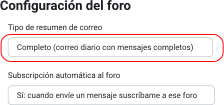
\includegraphics[height=0.25\textheight]{img/conf_pedco.pdf}
        \captionsetup{textfont=tiny,labelformat=empty}
        \caption{\url{https://pedco.uncoma.edu.ar/user/forum.php?id=3052&course=1}}
    \end{figure}
\end{itemize}

\end{frame}

\begin{frame}

    \frametitle{SIU Guaraní}
    \framesubtitle{\url{https://siufai.uncoma.edu.ar/}}

\begin{itemize}
    \item Sistema de Gestión Académica Guaraní.
    \item Inscribirse a materias y exámenes finales.
    \item Consultar el plan de la carrera.
    \item Consultar la historia académica.
    \item Actualizar datos personales.
\end{itemize}

\textbf{¡Si no están anotados en el \emph{SIU Guaraní} no están anotados a la
    materia!}

\end{frame}

\begin{frame}

    \frametitle{Metodología}
    \framesubtitle{Clases}

\begin{itemize}
    \item Clases teóricas:
    \begin{itemize}
        \item Virtuales: Jueves \textbf{13:00hs} a \textbf{15:00hs}.
        \item Presenciales: Viernes \textbf{10:00hs} a \textbf{12:00hs} (aula
            \textbf{13}).
    \end{itemize}
        \textbf{(Sólo hace falta asistir a una)}
    \item Clases prácticas:
    \begin{itemize}
        \item \textbf{Módulo I}: Martes \textbf{12:00hs} a \textbf{14:00hs}
            (aula \textbf{106}).
        \item \textbf{Módulo II}: Martes \textbf{15:00hs} a \textbf{17:00hs}
            (aulas \textbf{i1} y \textbf{i7}).
    \end{itemize}

\end{itemize}

\end{frame}

\begin{frame}

    \frametitle{Metodología}
    \framesubtitle{Condiciones de cursado}

\begin{itemize}
    \item Cursar la materia.
    \item Aprobar la materia:
        \begin{itemize}
            \item Por promoción.
            \item Por final regular.
            \item Por final libre.
        \end{itemize}
\end{itemize}

\end{frame}

\begin{frame}

    \frametitle{Metodología}
    \framesubtitle{Cursar la materia}

\begin{itemize}

    \item Aprobar los dos exámenes parciales (o sus respectivos
        recuperatorios).
    \item Cada parcial se aprueba teniendo un $60\%$ de las respuestas
        correctas.
    \item Se evalúan los contenidos prácticos y teóricos vistos en los
        trabajos prácticos.
    \item Si no se llega a aprobar un examen ni su recuperatorio, la o el
        estudiante queda libre.

\end{itemize}

\textbf{IMPORTANTE:} ¡La condición de cursada se pierde luego de 3 años!

\end{frame}

\begin{frame}

    \frametitle{Metodología}
    \framesubtitle{Aprobado por promoción}


Durante el cursado, si se aprueba el examen parcial con más del $80\%$:

\begin{itemize}
    \item Puede acceder al examen de promoción. Se valúa la teoría vista hasta
        el momento.
    \item Para rendir el segundo examen de promoción es necesario haber
        aprobado el primero.
    \item Se toman el mismo día que el recuperatorio del examen parcial.
\end{itemize}

\end{frame}

\begin{frame}

    \frametitle{Metodología}
    \framesubtitle{Aprobado por final regular}

Si se tiene la materia cursada:
\begin{itemize}
    \item Examen final regular: se evalúa la teoría.
    \item Clases de consulta: para dispersar dudas antes del examen.
\end{itemize}

\end{frame}

\begin{frame}

    \frametitle{Metodología}
    \framesubtitle{Aprobado por final libre}

Si no se tiene la materia cursada, ni se esta cursando:
\begin{itemize}
    \item Examen final libre:
        \begin{itemize}
            \item Parte práctica: se evalúan los temas de los trabajos
                prácticos.
            \item Parte teórica: solo se rinde si se aprobó con anterioridad
                la parte práctica. Se evaluan los temas vistos en teoria.
        \end{itemize}
\end{itemize}


\end{frame}

\begin{frame}

    \frametitle{Metodología}
    \framesubtitle{Dudas frecuentes}

\begin{itemize}

    \item Si se desaprueba el primer examen y su recuperatorio, ya no se puede
        cursar la materia en ese año.
    \item Si se obtiene una nota mayor a $80\%$ en el segundo examen, pero no
        se logro en el primero o no se aprobó el primer examen de promoción,
        no se puede rendir el segundo.
    \item Sólo se puede acceder a la promoción por medio de los exámenes
        parciales, no los recuperatorios.
    \item Los finales se aprueban con una nota mayor o igual a 4, pero eso no
        quiere decir que se tenga un $40\%$ de las respuestas correctas
        \footnote{\tiny Nosotros tampoco sabemos porqué es tan complicado}.

\end{itemize}

\end{frame}

\begin{frame}

    \frametitle{Finalizando}

\begin{itemize}

\item ¿Quiénes?

\item ¿Qué?

\item ¿Cuándo y dónde?

\item ¿Cómo?

\end{itemize}

\end{frame}

\begin{frame}

\title{¿Consultas?}
\maketitle

\end{frame}

\newcounter{lastPage}
\setcounter{lastPage}{\number\value{page}}

\begin{frame}%[allowframebreaks]

\frametitle{Atribuciones}

\bibliographystyle{abbrv}
\setbeamertemplate{bibliography item}{\insertbiblabel}
\tiny
\bibliography{refimg}
\end{frame}

\setcounter{page}{\number\value{lastPage}}

\end{document}
